\section{Rangga Putra Ramdhani}
\subsection{Buatlah librari fungsi (library dengan nama NPM bar.py) untuk plot dengan jumlah subplot adalah NPM mod 3 + 2}
\lstinputlisting[caption = fungsi bar., firstline=11, lastline=38]{src/6/Praktek/1174056/1174056_bar.py}
\begin{figure}[H]
	\includegraphics[width=9cm]{figures/6/Praktek/1174056/bar.png}
	\caption{Hasil dari fungsi bar.}
	\centering
\end{figure}

\subsection{Buatlah librari fungsi (library dengan nama NPM scatter.py) untuk plot dengan jumlah subplot NPM mod 3 + 2}
\lstinputlisting[caption = fungsi scatter., firstline=12, lastline=48]{src/6/Praktek/1174056/1174056_scatter.py}
\begin{figure}[H]
	\includegraphics[width=9cm]{figures/6/Praktek/1174056/scatter.png}
	\caption{Hasil dari fungsi scatter.}
	\centering
\end{figure}

\subsection{Buatlah librari fungsi (library dengan nama NPM pie.py) untuk plot dengan jumlah subplot NPM mod 3 + 2}
\lstinputlisting[caption = fungsi pie., firstline=11, lastline=64]{src/6/Praktek/1174056/1174056_pie.py}
\begin{figure}[H]
	\includegraphics[width=9cm]{figures/6/Praktek/1174056/pie.png}
	\caption{Hasil dari fungsi pie.}
	\centering
\end{figure}

\subsection{Buatlah librari fungsi (library dengan nama NPM plot.py) untuk plot dengan jumlah subplot NPM mod 3 + 2}
\lstinputlisting[caption = fungsi plot., firstline=8, lastline=30]{src/6/Praktek/1174056/1174056_plot.py}
\begin{figure}[H]
	\includegraphics[width=9cm]{figures/6/Praktek/1174056/plot.png}
	\caption{Hasil dari fungsi plot.}
	\centering
\end{figure}

\subsection{Screenshoot main}
\begin{figure}[H]
	\includegraphics[width=9cm]{figures/6/Praktek/1174056/kodinganmain.png}
	\caption{kodingan main.}
	\centering
\end{figure}

\subsection{Screenshoot mod}
\begin{figure}[H]
	\includegraphics[width=9cm]{figures/6/Praktek/1174056/kodingmod.png}
	\caption{kodingan mod.}
	\centering
\end{figure}

\begin{figure}[H]
	\includegraphics[width=9cm]{figures/6/Praktek/1174056/hasilmod.png}
	\caption{hasil mod.}
	\centering
\end{figure}

\subsection{Pengecekan Plagiarisme Praktek}
\begin{figure}[H]
	\includegraphics[width=9cm]{figures/6/Praktek/1174056/Plagiatpraktek.png}
	\centering
\end{figure}

\subsection{Ketrampilan Penanganan Error}
\textbf{Tuliskan peringatan error yang didapat dari mengerjakan praktek ketiga ini, dan jelaskan cara penanganan error tersebut. dan Buatlah satu fungsi yang menggunakan gunakan try except untuk menanggulangi error tersebut}

Peringatan error yang saya temui pada praktek Chapter 6 ini, adalah:
\begin{itemize}
	\item Name Error
	NameError adalah exception yang terjadi ketika kode melakukan eksekusi terhadap local name atau global name yang tidak terdefinisi oleh perangkat. Solusi yang dapat dilakukan adalah dengan memastikan variabel atau fungsi yang dipanggil ada atau tidak salah ketik.
	
	\item Syntax Errors
	Syntax Errors adalah suatu keadaan saat  terjadi kesalahan penulisan pada kode python. Cara memperbaikinya adalah dengan memperbaiki penulisan kode yang salah.
	
	\item Type Error
	TypeError adalah exception yang terjadi pada saat dilakukannya eksekusi terhadap suatu operasi atau fungsi dengan type object yang tidak sesuai. Cara yang dilakukan untuk mengatasinya error ini adalah mengkoversi varibelnya sesuai dengan tipe data yang akan digunakan.
\end{itemize}

\textbf{Penanggulangan Error menggunakan Try Except}
\lstinputlisting[caption = Penanggulangan error menggunakan Try Except., firstline=8, lastline=25]{src/6/Praktek/1174056/1174056_error.py}

\subsection{Pengecekan Plagiarisme Penanganan Error}
\begin{figure}[H]
	\includegraphics[width=9cm]{figures/6/Praktek/1174056/Plagiarismeerror.png}
	\centering
\end{figure}
%%%%%%%%%%%%%%%%%%%%%%%%%%%%%%%%%%%%%%%%%%%%%%%%%%%%%%%%%%%
\section{Liyana Majdah Rahma 1174039}
\subsection{Praktek}
\subsubsection{Soal No. 1}
\hfill \break
Buatlah librari fungsi (file terpisah/library dengan nama NPMbar.py) untuk plot dengan jumlah subplot adalah NPM mod 3 + 2!

\hfill \break
\textbf{Kode Program}

\lstinputlisting[caption = Kode program membuat fungsi Bar Plot menggunakan Matplotlib., firstline=1, lastline=21]{src/6/Praktek/1174039/1174039_bar.py}

\hfill \break
\textbf{Hasil Compile}

\begin{figure}[H]
	\includegraphics[width=12cm]{figures/6/Praktek/1174039/p1.png}
	\centering
	\caption{Hasil compile membuat fungsi Bar Plot menggunakan Matplotlib.}
\end{figure}

\subsubsection{Soal No. 2}
\hfill \break
Buatlah librari fungsi (file terpisah/library dengan nama NPMscatter.py) untuk plot dengan jumlah subplot NPM mod 3 + 2!

\hfill \break
\textbf{Kode Program}

\lstinputlisting[caption = Kode program membuat fungsi Scatter Plot menggunakan Matplotlib., firstline=1, lastline=23]{src/6/Praktek/1174039/1174039_scatter.py}

\hfill \break
\textbf{Hasil Compile}

\begin{figure}[H]
	\includegraphics[width=12cm]{figures/6/Praktek/1174039/p2.png}
	\centering
	\caption{Hasil compile membuat fungsi Scatter Plot menggunakan Matplotlib.}
\end{figure}

\subsubsection{Soal No. 3}
\hfill \break
Buatlah librari fungsi (file terpisah/library dengan nama NPMpie.py) untuk plot dengan jumlah subplot NPM mod 3 + 2!

\hfill \break
\textbf{Kode Program}

\lstinputlisting[caption = Kode program membuat fungsi Pie Plot menggunakan Matplotlib., firstline=1, lastline=23]{src/6/Praktek/1174039/1174039_pie.py}

\hfill \break
\textbf{Hasil Compile}

\begin{figure}[H]
	\includegraphics[width=12cm]{figures/6/Praktek/1174039/p3.png}
	\centering
	\caption{Hasil compile membuat fungsi Pie Plot menggunakan Matplotlib.}
\end{figure}

\subsubsection{Soal No. 4}
\hfill \break
Buatlah librari fungsi (file terpisah/library dengan nama NPMplot.py) untuk plot dengan jumlah subplot NPM mod 3 + 2

\hfill \break
\textbf{Kode Program}

\lstinputlisting[caption = Kode program membuat fungsi Plot menggunakan Matplotlib., firstline=1, lastline=23]{src/6/Praktek/1174039/1174039_plot.py}

\hfill \break
\textbf{Hasil Compile}

\begin{figure}[H]
	\includegraphics[width=12cm]{figures/6/Praktek/1174039/p4.png}
	\centering
	\caption{Hasil compile membuat fungsi Plot menggunakan Matplotlib.}
\end{figure}


\subsection{Penanganan Error}
Tuliskan  peringatan  error  yang  didapat  dari  mengerjakan  praktek  keenam  ini, dan  jelaskan  cara  penanganan  error  tersebut. dan  Buatlah  satu  fungsi  yang menggunakan try except untuk menanggulangi error tersebut.

\hfill \break
Peringatan error di praktek kelima ini, yaitu:
\begin{itemize}
	\item Syntax Errors
	Syntax Errors adalah suatu keadaan saat kode python mengalami kesalahan penulisan. Solusinya adalah memperbaiki penulisan kode yang salah.
	
	\item Name Error
	NameError adalah exception yang terjadi saat kode melakukan eksekusi terhadap local name atau global name yang tidak terdefinisi. Solusinya adalah memastikan variabel atau function yang dipanggil ada atau tidak salah ketik.
	
	\item Type Error
	TypeError adalah exception yang akan terjadi apabila pada saat dilakukannya eksekusi terhadap suatu operasi atau fungsi dengan type object yang tidak sesuai. Solusi dari error ini adalah mengkoversi varibelnya sesuai dengan tipe data yang akan digunakan.
\end{itemize}
\hfill \break
Fungsi yang menggunakan try except untuk menanggulangi error.

\hfill \break
\textbf{Kode Program}

\lstinputlisting[caption = Kode program membuat fungsi penanganan error., firstline=161, lastline=178]{src/6/Praktek/1174039/1174039.py}

\hfill \break
\textbf{Hasil Compile}

\begin{figure}[H]
	\includegraphics[width=12cm]{figures/6/Praktek/1174039/error.png}
	\centering
	\caption{Hasil compile membuat fungsi penanganan error.}
\end{figure}

\subsection{Screenshoot Plagiat}
\begin{figure}[H]
	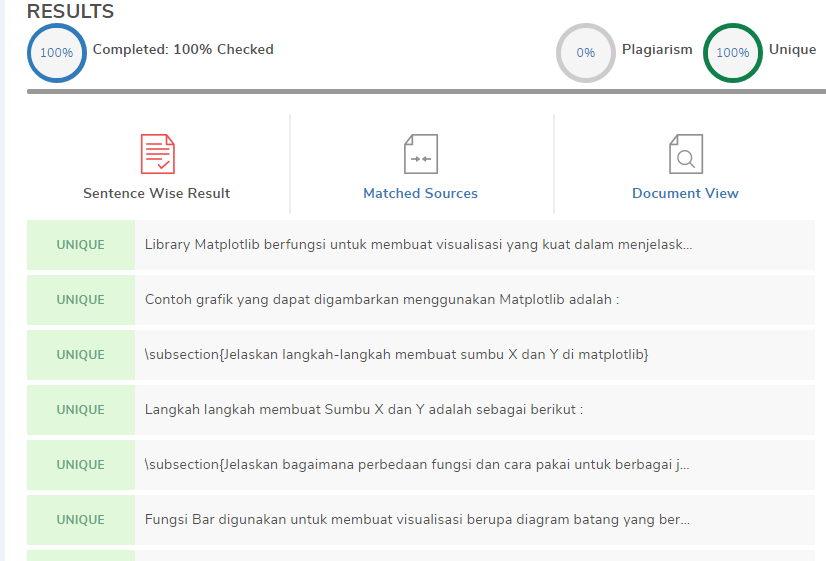
\includegraphics[width=12cm]{figures/6/Praktek/1174039/plagiat.png}
	\centering
\end{figure}
\subsection{Screenshoot Kode Program}
\begin{figure}[H]
	\includegraphics[width=9cm]{figures/6/Praktek/1174039/c1.png}
	\centering
\end{figure}
\begin{figure}[H]
	\includegraphics[width=9cm]{figures/6/Praktek/1174039/c2.png}
	\centering
\end{figure}
\begin{figure}[H]
	\includegraphics[width=9cm]{figures/6/Praktek/1174039/c3.png}
	\centering
\end{figure}
\begin{figure}[H]
	\includegraphics[width=9cm]{figures/6/Praktek/1174039/c4.png}
	\centering
\end{figure}
\begin{figure}[H]
	\includegraphics[width=9cm]{figures/6/Praktek/1174039/c5.png}
	\centering
\end{figure}
\begin{figure}[H]
	\includegraphics[width=9cm]{figures/6/Praktek/1174039/c6.png}
	\centering
\end{figure}
\begin{figure}[H]
	\includegraphics[width=9cm]{figures/6/Praktek/1174039/c7.png}
	\centering
\end{figure}
\begin{figure}[H]
	\includegraphics[width=9cm]{figures/6/Praktek/1174039/c8.png}
	\centering
\end{figure}
\begin{figure}[H]
	\includegraphics[width=9cm]{figures/6/Praktek/1174039/c9.png}
	\centering
\end{figure}
\begin{figure}[H]
	\includegraphics[width=9cm]{figures/6/Praktek/1174039/c10.png}
	\centering
\end{figure}

\section{Teddy Gideon Manik}
\subsubsection{Soal No. 1}
\hfill \break
Buatlah librari fungsi (file terpisah/library dengan nama NPMbar.py) untuk plot dengan jumlah subplot adalah NPM mod 3 + 2!

\hfill \break
\textbf{Kode Program}

\lstinputlisting[caption = Kode program membuat fungsi Bar Plot menggunakan Matplotlib., firstline=1, lastline=21]{src/6/Praktek/1174038/1174038_bar.py}

\hfill \break
\textbf{Hasil Compile}

\begin{figure}[H]
	\includegraphics[width=12cm]{figures/6/Praktek/1174038/p1.png}
	\centering
	\caption{Hasil compile membuat fungsi Bar Plot menggunakan Matplotlib.}
\end{figure}

\subsubsection{Soal No. 2}
\hfill \break
Buatlah librari fungsi (file terpisah/library dengan nama NPMscatter.py) untuk plot dengan jumlah subplot NPM mod 3 + 2!

\hfill \break
\textbf{Kode Program}

\lstinputlisting[caption = Kode program membuat fungsi Scatter Plot menggunakan Matplotlib., firstline=1, lastline=23]{src/6/Praktek/1174038/1174038_scatter.py}

\hfill \break
\textbf{Hasil Compile}

\begin{figure}[H]
	\includegraphics[width=12cm]{figures/6/Praktek/1174038/p2.png}
	\centering
	\caption{Hasil compile membuat fungsi Scatter Plot menggunakan Matplotlib.}
\end{figure}

\subsubsection{Soal No. 3}
\hfill \break
Buatlah librari fungsi (file terpisah/library dengan nama NPMpie.py) untuk plot dengan jumlah subplot NPM mod 3 + 2!

\hfill \break
\textbf{Kode Program}

\lstinputlisting[caption = Kode program membuat fungsi Pie Plot menggunakan Matplotlib., firstline=1, lastline=23]{src/6/Praktek/1174038/1174038_pie.py}

\hfill \break
\textbf{Hasil Compile}

\begin{figure}[H]
	\includegraphics[width=12cm]{figures/6/Praktek/1174038/p3.png}
	\centering
	\caption{Hasil compile membuat fungsi Pie Plot menggunakan Matplotlib.}
\end{figure}

\subsubsection{Soal No. 4}
\hfill \break
Buatlah librari fungsi (file terpisah/library dengan nama NPMplot.py) untuk plot dengan jumlah subplot NPM mod 3 + 2

\hfill \break
\textbf{Kode Program}

\lstinputlisting[caption = Kode program membuat fungsi Plot menggunakan Matplotlib., firstline=1, lastline=23]{src/6/Praktek/1174038/1174038_plot.py}

\hfill \break
\textbf{Hasil Compile}

\begin{figure}[H]
	\includegraphics[width=12cm]{figures/6/Praktek/1174038/p4.png}
	\centering
	\caption{Hasil compile membuat fungsi Plot menggunakan Matplotlib.}
\end{figure}


\subsection{Penanganan Error}
Tuliskan  peringatan  error  yang  didapat  dari  mengerjakan  praktek  keenam  ini, dan  jelaskan  cara  penanganan  error  tersebut. dan  Buatlah  satu  fungsi  yang menggunakan try except untuk menanggulangi error tersebut.

\hfill \break
Peringatan error di praktek kelima ini, yaitu:
\begin{itemize}
	\item Syntax Errors
	Syntax Errors adalah suatu keadaan saat kode python mengalami kesalahan penulisan. Solusinya adalah memperbaiki penulisan kode yang salah.
	
	\item Name Error
	NameError adalah exception yang terjadi saat kode melakukan eksekusi terhadap local name atau global name yang tidak terdefinisi. Solusinya adalah memastikan variabel atau function yang dipanggil ada atau tidak salah ketik.
	
	\item Type Error
	TypeError adalah exception yang akan terjadi apabila pada saat dilakukannya eksekusi terhadap suatu operasi atau fungsi dengan type object yang tidak sesuai. Solusi dari error ini adalah mengkoversi varibelnya sesuai dengan tipe data yang akan digunakan.
\end{itemize}
\hfill \break
Fungsi yang menggunakan try except untuk menanggulangi error.

\hfill \break
\textbf{Kode Program}

\lstinputlisting[caption = Kode program membuat fungsi penanganan error., firstline=161, lastline=178]{src/6/Praktek/1174038/1174038.py}

\hfill \break
\textbf{Hasil Compile}

\begin{figure}[H]
	\includegraphics[width=12cm]{figures/6/Praktek/1174038/error.png}
	\centering
	\caption{Hasil compile membuat fungsi penanganan error.}
\end{figure}

